\documentclass{article} % For LaTeX2e
\usepackage{nips15submit_e,times}
\usepackage{graphicx}
\usepackage{amsmath}
\usepackage{hyperref}
\usepackage{url}
\usepackage{float}
%\documentstyle[nips14submit_09,times,art10]{article} % For LaTeX 2.09


\title{Breast Cancer Detection Using AI}


\author{
Ken Chen\thanks{} \\
Department of Computer Science and Software Engineering\\
Auburn University\\
345 W Magnolia Ave, Auburn, AL 36849 \\
\texttt{kzc0068@auburn.edu} \\
\And
Donglai Liu \\
Department of Computer Science and Software Engineering \\
Auburn University\\
Address 345 W Magnolia Ave, Auburn, AL 36849\\
\texttt{dzl0066@auburn.edu} \\
\AND
Junyao Yang \\
Department of Industrial and Systems Engineering \\
Auburn University\\
345 W Magnolia Ave, Auburn, AL 36849 \\
\texttt{jzy0040@auburn.edu} \\
}

% The \author macro works with any number of authors. There are two commands
% used to separate the names and addresses of multiple authors: \And and \AND.
%
% Using \And between authors leaves it to \LaTeX{} to determine where to break
% the lines. Using \AND forces a linebreak at that point. So, if \LaTeX{}
% puts 3 of 4 authors names on the first line, and the last on the second
% line, try using \AND instead of \And before the third author name.

\newcommand{\fix}{\marginpar{FIX}}
\newcommand{\new}{\marginpar{NEW}}

%\nipsfinalcopy % Uncomment for camera-ready version

\begin{document}


\maketitle

\begin{abstract}
Scientific evidences show that treatments can be more successful when identify breast cancer at early stages of the disease. Despite the existence of screening programs worldwide, correct identify accuracy is still suffering from high rates of false positives and false negatives. In this project, we will try to build an artificial intelligence system that is capable to detect abnormal cells at early stage of the disease. To assess it's performance, multiple comparisons are performed, for example, human vs machine and comparison among AI models. According to our experiments, we find that the Neural Network outperformed to other models. However, our baseline models and CNN also provide high accuracy capabilities to do classification. We conclude that AI will provide a competitive solution to healthcare industry. 
\end{abstract}

\section{Introduction}
Breast Cancer's causes are multifactorial and one million women are newly diagnosed with breast cancer every year. Machine learning is a powerful tool and algorithms that facilitate prediction, pattern recognition and classification. In this project, we develop two algorithms of machine learning for breast cancer classification, Neural Network and Convolutional Neural Network. We also develop two baseline models for comparison purpose, K Nearest Neighbors and Naive Bayes Classifier, and they are widely used  as baseline in this area. The Wisconsin Breast Cancer Database provides an easy accessible and well organized database and we split it into train and test samples. Neural Network can classify both linear space and nonlinear space, and two layers Neural Network can have a good approximation to any function with different setting on activation function. Convolutional Neural Network can explore features in the database and learn internal relation between features. Then, it will generate more features to use in prediction. This self-learning capability makes Convolutional Neural Network as Deep learning category. The purpose of this project is studying and developing effective machine learning based model for cancer detection using binary classification data set. 

\section{Literature Review}
\label{gen_inst}
Support Vector Machine(SVM), Decision Tree(C4.5), Naive Bayes(NB) and k Nearest Neighbors (k-NN) on the Wisconsin Breast Cancer (original) dataset are conducted[1]. k Nearest Neighbors (k-NN) is used as baseline method. Naive Bayes(NB) classifier and k nearest neighbor(KNN) are applied for breast cancer classification[2]. More recently, deep learning methods have been researched to solve anomaly detection problems since they do not require explicit feature construction unlike previously methods[3].


\section{Methods}
\label{headings}

First task is choosing a baseline algorithm. Based on our literature, KNN and Naive Bayes algorithm are most well studied model in literature. And they are all very basic machine learning algorithm. All other methods we used will be compare to our baseline algorithms on algorithm performance. We are aiming to develop a system that can outperform comparing to our baseline. When choose our baseline methods, we need to keep one thing in mind. The linearity of the dataset is not the main focus in this project. So when we choose machine learning algorithm, we will focus on those algorithm that can handle both linear and nonlinear space. As a result, the algorithms in this project are KNN, NBC, NN and CNN.

\subsection{Dataset}
Wisconsin Breast Cancer (original) dataset will be used. Dataset was designed for binary classification. There are 699 instances and 10 attributes with missing values. All attributes are integer values. There are 31 features in this dataset. We have a high dimension problem. We will clean the data by delete the patient id and delete the missing values in our study. And it results in 569 observations after cleaning. Dataset is randomly split with ratio 0.2 between training and testing sample size. First, we preform a correlation check using Heatmap in figure 1 to have an idea about the relation among features. Then, as we mentioned before that the missing values are ignored. Link to our dataset is provided in Appendix. 

\begin{figure}[H]
\begin{center}
%\framebox[4.0in]{$\;$}
\fbox{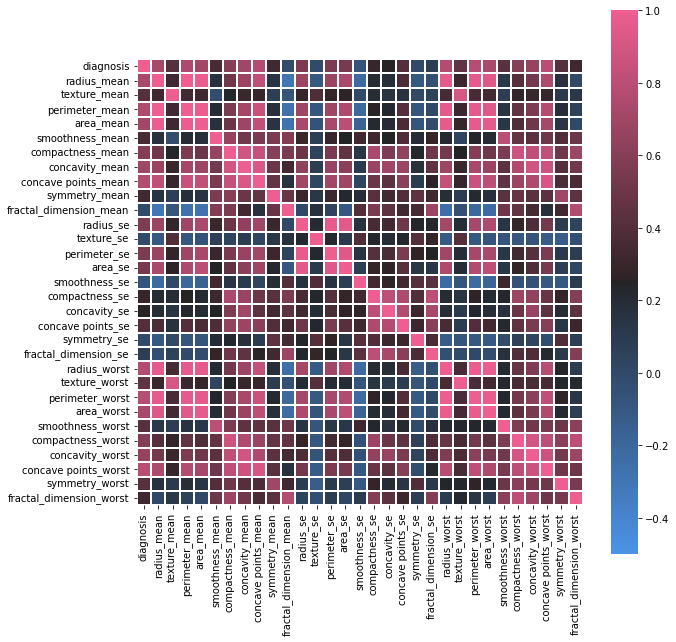
\includegraphics[width = 8cm, height = 8cm]{heatmap.png}}
\caption{Dataset Heatmap on Features}
\end{center}
\end{figure}

\subsection{K nearest neighbors}
The KNN algorithm is used to detect cancer as baseline. Given N training vector, suppose we
have A and Z as training vectors in this bi-dimensional features space, we want to classify c which is feature vector. Classifying c depends on its k neighbors, and the majority vote, k is a positive integer. Tuning parameter k is explained and analyzed in section Experiment. We will use learning curve to analyze k and make our decision according to the accuracy. In our study, two distance definition is used in this project, Euclidean and Manhattan distance. Euclidean and Manhattan distance are defined in equations 1 and 2, respectively. Theoretically, Manhattan distance is preferred over the Euclidean distance metric as the dimension of the data increase. This occur due to something known as the curse of the dimensionality[4]. To study KNN, we will verify this theory through our experiments.

\begin{equation}
 d\left(p,q\right) = \sqrt {\sum _{i=1}^{n}  \left( q_{i} - p_{i}\right)^2 } 
\end{equation}


\begin{equation}
 d\left(p,q\right) = \sum _{i=1}^{n} \lvert \left( q_{i} - p_{i}\right) \rvert
\end{equation}

\subsection{Naive Bayes}
A Bayesian method is a basic mathematical model in probabilities and statistics. It can be defined as a framework to model decisions. In NBC, variables are conditionally independent. NBC can be used on data that directly influence each other to determine a model. From known training compounds, active (D) and inactive (H), Given representation B, the conditional probability distribution P(B/D) and P(B/H) are estimated, respectively. Bayesian classifiers are additionally well adapted for ranking of compound databases all with consideration to probability of activity.
Bayesian classifiers use Bayes theorem which is defined in equation 3.
\begin{equation}
p(h|d) = \frac{p(d|h)p(h)}{p(d)}
\end{equation}


\subsection{Neural Network}
An NN is a machine learning algorithm suitable for different tasks including classification, prediction and visualization. Furthermore, an NN is suitable or multi-disciplinary tasks with the use of multiple types of data which may be unstructured, semi-structured and structured data. Consider that our dateset may not be a linear separate-able space which means linear classifier, like SVM and Perceptron classifier may not perform well. Then NN will be a good candidate to resolve this issue. Because theoretically, Ann with 2 hidden layers is capable to approximate variety problems. We will implement exactly 2 hidden layers Neural Network and the structure is showing in figure 2. The number of neurons in hidden layers will be one of our interested parameter. And we will also study train and test split ratio regarding the accuracy of prediction. The analysis and explanation are conducted in Experiments section.

\begin{figure}[H]
\begin{center}
%\framebox[4.0in]{$\;$}
\fbox{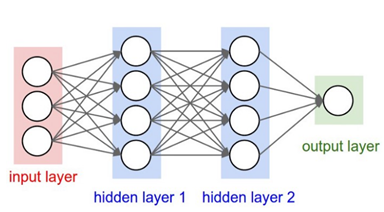
\includegraphics[width = 8cm, height = 5cm]{NN_structure.jpg}}
\caption{2 Layers Neural Network}
\end{center}
\end{figure}

\subsection{Convolutional Neural Network}

Convolutional neural network(CNN) are the quickest rising areas in healthcare industry. CNN brings to research on medical imaging is not restricted to deep CNN for extraction of the imaging feature. CNN is one of well known deep learning algorithm. It takes in an input image, assign importance to variable feature or aspect, extract learnable features in the image and be able to differentiate on from the other. The objective of convolution operation is to extract the high level features such as edges from the input image. We will try to build an neural network with convolutional layer to detect breast cancer cells. The structure of CNN is showing in figure 3. It basically has two states, feature learning and Classification. And these two stages are separated by a flatten layer. 

\begin{figure}[H]
\begin{center}
%\framebox[4.0in]{$\;$}
\fbox{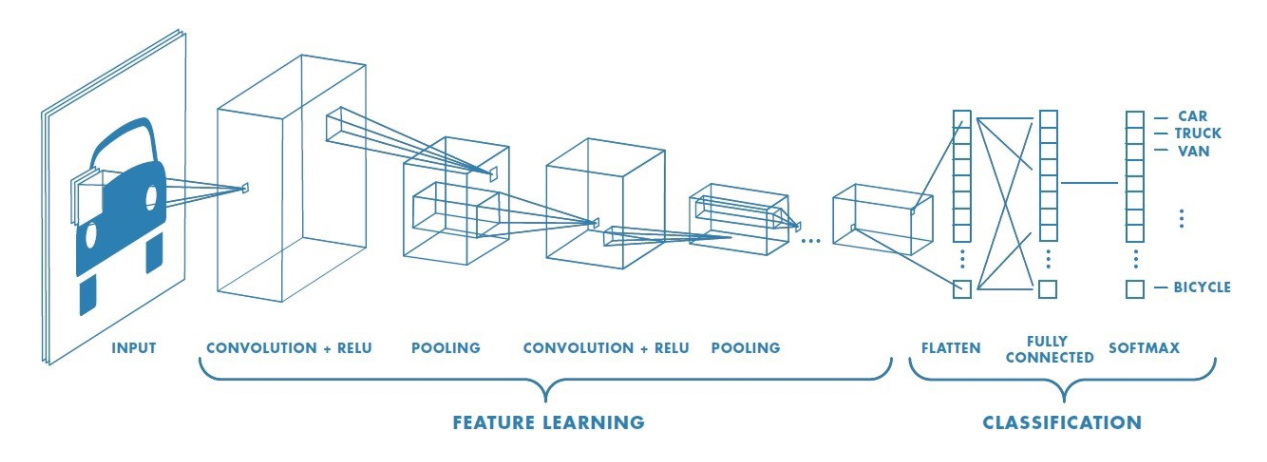
\includegraphics[width = 12cm, height = 5cm]{CNN_structure.png}}
\caption{Convolutional Neural Network}
\end{center}
\end{figure}

\section{Experiments and Analysis}
In this section, we will show our experiments on these four models with parameter settings. The final results are showing in table .And we will briefly discuss the comparison among these experiment results.
\subsection{KNN Baseline}
In our baseline model, KNN is studied by the variation of k and distance metric. k is number of nearest neighbors compares towards our test sample. We initialize it with a small integer 5 and apply learning curve analysis in range 5, 30. The parameters are showing in table 1. The results are showing in table 4. The learning curve analysis regarding k and accuracy is showing in figure 4. The learning curve analysis between distance metric and accuracy is showing in figure 5.

\begin{table}[H]
\caption{Knn Settings}
\begin{center}
\begin{tabular}{lll}
\multicolumn{1}{c}{\bf PARAMETER}  &\multicolumn{1}{c}{\bf DESCRIPTION}  &\multicolumn{1}{c}{\bf Settings}
\\ \hline \\
k          & Number of Closest Neighbors & Range(5, 30) \\
Distance Metric   & Euclidean and Manhattan &Equation 1, 2 \\
\end{tabular}
\end{center}
\end{table}

The learning curve analysis in Figure 4 shows that when k is in range 15 to 18. Both distance metric return a good accuracy. So we finally chose 16 as our k value. Indeed that, we confirm through our experiments that Manhattan distance is outperformed than Euclidean distance. This can be easily explained by when we are handling outliners. Euclidean distance will enlarge the effects of those value by square it. But Manhattan distance doesn't have such square operation so that it usually outperformed in high dimensional problem and it's exactly what we have in this project. The training and testing sample ratio do not really show significant difference, Figure 5. We will simply use the ratio we found in Neural Network model which is 0.2 and it's explained in Neural Network subsection. 

\begin{figure}[H]
\begin{center}
%\framebox[4.0in]{$\;$}
\fbox{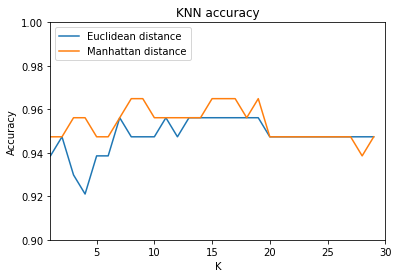
\includegraphics[width = 8cm, height = 5cm]{KNN_k_lc.png}}
\caption{KNN k Learn Curve}
\end{center}
\end{figure}

\begin{figure}[H]
\begin{center}
%\framebox[4.0in]{$\;$}
\fbox{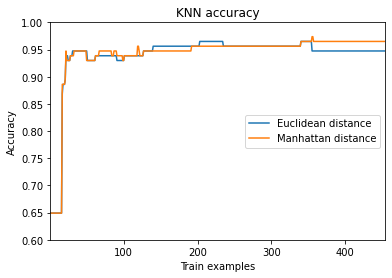
\includegraphics[width =8cm, height = 5cm]{KNN_distance.png}}
\caption{KNN Distance Metric Learning Curve}
\end{center}
\end{figure}

\subsection{Naive Bayes Classifier}
Naive Bayes methods are a set of supervised learning algorithms based on applying Bayes’ theorem with the “naive” assumption of conditional independence between every pair of features given the value of the class variable. There is not many flexibilities to tune the parameter in NBC. The default setting is applied. NBC usually have an initial hypothesis that the features' value are normal distributed. So we perform a sample check showing some of the features and it is shown in figure 6. There are still some feature with a high skewness according to their distribution. So we will perform a normalization on features for NBC model. The performance results are showing in table 4. The learning curve analysis between ratio and accuracy is showing in figure 7. It helps us study the behavior of NBC model on the training and testing sample split ratio. It turns out that the accuracy converges in the training size around 300. So we will apply the same ratio as Neural Network, 0.2. As a result, we will use the train test split ratio 0.2 consistently throughout our project. 

\begin{figure}[H]
\begin{center}
%\framebox[4.0in]{$\;$}
\fbox{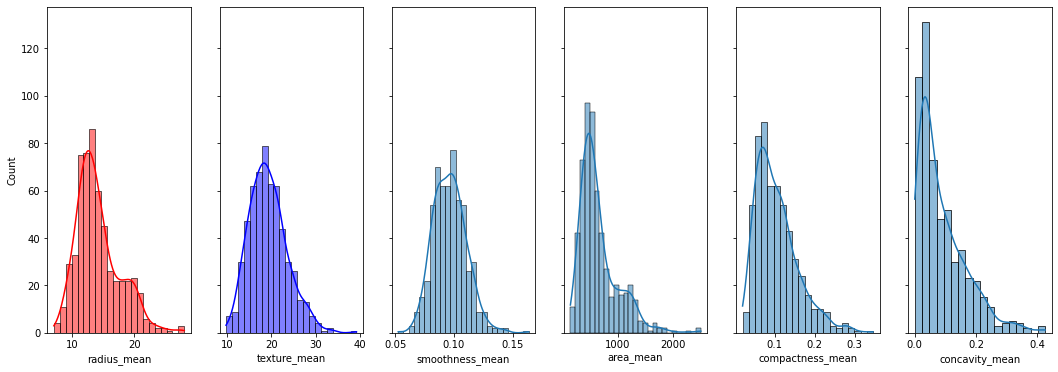
\includegraphics[width = 12cm, height = 5cm]{NBC_skewness_check.png}}
\caption{NBC Skewness Check}
\end{center}
\end{figure}

\begin{figure}[H]
\begin{center}
%\framebox[4.0in]{$\;$}
\fbox{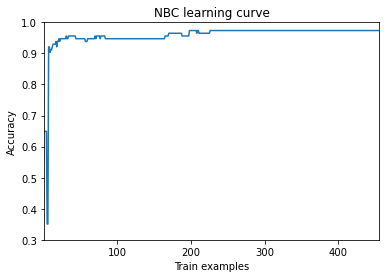
\includegraphics[width = 8cm, height = 5cm]{NBC_lc.png}}
\caption{NBC Learning Curve}
\end{center}
\end{figure}


\subsection{Neural Network}
Neural Network requires normalization on the dataset. We use standard normalization method to perform this task and all sample feature values are in range 0 to 1. As neural network needs sufficient amount of training samples to achieve good accuracy in generalization. We need to decide the ratio between the size of training and testing samples. Then, the next task is to decide how many neurons in each hidden layer. There is nontrivial method to perform this task. We will apply learning curve retarding the accuracy of model to do this task. The setting is showing in table 2. The activation function we used is Rectified Linear Unit(ReLU). The results are showing in table 4. The learning curve analysis between ratio and accuracy is showing in figure 8. Theoretically, Neural Network prefer more training samples to achieve a good generalization on test set. But we have a small dataset available with 699 observations and there are only 569 left over after data cleaning. As it is showed in figure 8, the accuracy is still growing with more training data involved. But to balance the size between training and test samples, we will use 0.2 as our ratio and it's 455 in training and 114 in testing samples. 

\begin{table}[H]
\caption{Neural Network Settings}
\begin{center}
\begin{tabular}{lll}
\multicolumn{1}{c}{\bf PARAMETER}  &\multicolumn{1}{c}{\bf DESCRIPTION}  &\multicolumn{1}{c}{\bf Settings}
\\ \hline \\
Ratio         &Train and Test Size Ratio & Range(0, 1) \\
Neuron   &Hidden Layer Neurons & Range(5, 20)\\
\end{tabular}
\end{center}
\end{table}

\begin{figure}[H]
\begin{center}
%\framebox[4.0in]{$\;$}
\fbox{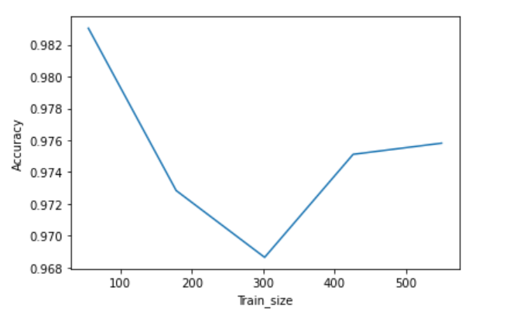
\includegraphics[width = 8cm, height = 5cm]{NN_lc.png}}
\caption{NN Learning Curve}
\end{center}
\end{figure}


\subsection{Convolutional Neural Network}
Convolutional Neural Network contains feature learning stage and classification stage. In feature learning stage, we use the first 6 layers in table 3. For the prediction stage, we use fully connected neural network with ReLU activation function as what we implemented in our Neural Network. The dimension of each layers are showing in table 3 as well. 

\begin{table}[H]
\caption{CNN Settings}
\begin{center}
\begin{tabular}{ll}
\multicolumn{1}{c}{\bf Layers}  &\multicolumn{1}{c}{\bf Shape}
\\ \hline \\
Conv1d    &(None, 29, 32) \\
Batch normalization  &(None, 29, 32)\\
Dropout   &(None, 29, 32)\\
Conv1d 1  &(None, 28, 64)\\
Batch normalization 1  &(None, 28, 64)\\
Dropout 1 & (None, 28, 64)\\
Flatten   & (None, 1792)\\
Dense   & (None, 64)\\
Dropout 2 & (None, 64)\\
Dense 1   & (None, 1)\\
\end{tabular}
\end{center}
\end{table}

In CNN, we are interested in the training epoch settings. We will use the range from 1 to 50 regarding the performance of our model. As showing in the figure, we are underfitting the model at the begining of your epoch. And it converges somewhere in range 40 to 50. The learning curve analysis between epoch and accuracy is showing in figure 9 and the loss is showing in figure 10. Between 40 and 50, we will use 45 as our epoch parameter. The performance results are showing in table 4.

\begin{figure}[H]
\begin{center}
%\framebox[4.0in]{$\;$}
\fbox{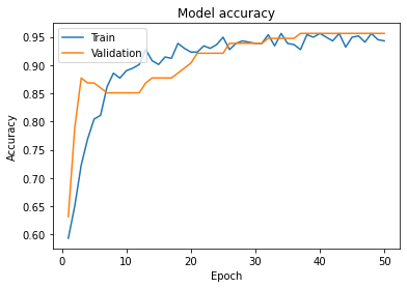
\includegraphics[width = 8cm, height = 5cm]{CNN_lc.png}}
\caption{CNN Learning Curve}
\end{center}
\end{figure}



\begin{figure}[H]
\begin{center}
%\framebox[4.0in]{$\;$}
\fbox{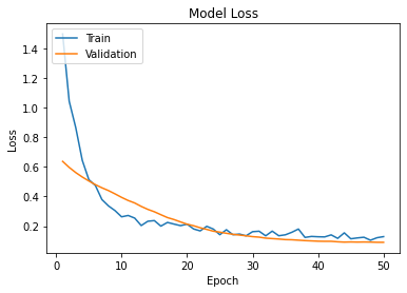
\includegraphics[width = 8cm, height = 5cm]{CNN_loss.png}}
\caption{CNN Learning Curve}
\end{center}
\end{figure}

The performance matrix is showing below. We randomly split the dataset using random state parameter from 0 to 40. The best model we found is the Naive Bayes model in terms of average accuracy. KNN turns out to be better performed to use Manhattan distance. It meets our expectation and we confirm this behavior. Naive Bayes performs good and stable with less parameter to tune which makes it a robust classifier. NN needs more samples to train and takes longer time to run on average. But it turns out to be our best model. We were expecting CNN to be the best model. But due to the complexity of CNN, we are not able to fully tune the model. Because there are too many parameters in the model. Future study is expected on CNN model to do this task. And we also need to find a bigger dataset to perform our training. 

\begin{table}[H]
\caption{Model Performance}
\begin{center}
\begin{tabular}{ll}
\multicolumn{1}{c}{\bf Model}  &\multicolumn{1}{c}{\bf Accuracy}
\\ \hline \\
KNN Euclidean    & 0.938 \\
KNN Manhattan  & 0.947\\
Naive Bayes   & 0.953\\
Neural Network  & 0.963\\
Convolutional NN  & 0.956\\
\end{tabular}
\end{center}
\end{table}



\section{Conclusion}
We build 4 models to perform binary classification regarding on cancer cell detection. And they all perform good on accuracy, more than 0.9. Machine learning algorithms provide a new perspective and robust solution to our project. Neural Network is actually a robust and universal model to solve variety problems. Although KNN is used as baseline model in many problems, it doesn't mean it performs badly. It actually provides a good threshold in model building and research. And we conclude that machine learning has huge potentials in healthcare industry. Future study needs to be conduct in dataset collection, feature study and more complex deep learning algorithm. We need a fast and robust model which can perform a good detection on cancer cells in terms of accuracy. Moreover, we want a model to detect cancer cells at their early stage which means more possible to have a successful treatment. So cancer cells in the early stage are preferred in the dataset. 
\subsubsection*{References}

\small{

[1] Hiba Asria. \& Hajar Mousannif. \& Hassan Al Moatassime.(2016)Using Machine Learning Algorithms for Breast Cancer Risk Prediction and Diagnosis. In The 7th International Conference on Ambient Systems, Networks and Technologies (ANT 2016) {\it Procedia Computer Science} vol 83, page 1064-1069. ISSN 1877-0509.


[2] Meriem AMRANE. \& Saliha OUKID. (2018) Breast Cancer Classification Using Machine Learning. {\it 2018 Electric Electronics, Computer Science, Biomedical Engineerings' Meeting 10.1109/EBBT.2018.8391453}.

[3] Li Shen. \& Laurie R. Margolies. (2019) Deep Learning to Improve Breast
Cancer Detection on Screening Mammography. {\it Scientific Reports} volume 9, Article number: 12495.

[4] Charu C. Aggarwal. \& Alexander Hinneburg. \& Daniel A. Keim. (2001) On the Surprising Behavior of Distance Metrics in High Dimensional Space. {\it International Conference on Database Theory} ICDT 2001: Database Theory — ICDT 2001 pp 420-434.
}

\end{document}
